\documentclass[12pt,a4paper]{article}
\usepackage[T2A]{fontenc}
\usepackage[utf8]{inputenc}
\usepackage[russian]{babel}
\usepackage{graphicx, setspace, longtable}

\usepackage[
top = 1.25cm, 
bottom = 2.0cm]{geometry}

\begin{document}
\begin{titlepage} 
	\centering
    % HEADER
	{
        \scshape
        Федеральное государственное автономное образовательное учреждение высшего образования
        \par
        \textbf{«Научно-образовательная корпорация ИТМО»}
        \par
        \vspace*{1cm}
        Факультет Программной Инженерии и Компьютерной Техники
        \par
    }
    % LOGO
    \vspace*{0.6cm}
    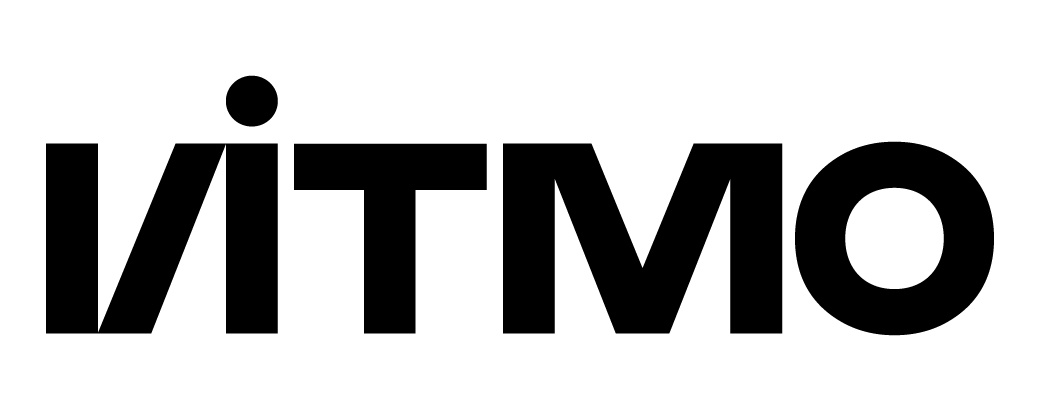
\includegraphics[width=\textwidth]{logo.png}
    % LAB INFO
    {
        \Large
        \textbf{Лабораторная работа по физике №1}
        \par
        \normalsize
        \vspace*{0.75cm}
        \textbf{Исследование распределения случайной величины}
        \par
    }
    \vfill
    % СREDITS
    \hfill\begin{minipage}{\dimexpr\textwidth-7.8cm}
        \textbf{Выполнили:}\par
        Степанов Арсений Алексеевич\par
        Выдра Андрей Михайлович\par
        \vspace*{0.15cm}
        \textbf{Группа:}\par
        ФИЗ ПИиКТ БАЗ 3.4.1\par
        \vspace*{0.15cm}
        \textbf{Преподаватель:}\par
        Пулькин Николай Сергеевич\par
    \end{minipage}
    \vfill
    Санкт-Петербург, \the\year{}г.
\end{titlepage}  
\section{Цели работы}
Произвести исследование случайной величины и построить соответствующие схемы и графики на основе произведённых измерений
\section{Схема установки}
Пара секундомеров, используемых для измерения интервалов времени
\subsection{Измерительные приборы}
\hfill\break
\begin{tabular}{|c|c|c|c|c|}
    \hline
    № & Наименование & Тип & Используемый диапазон & Погрешность \\
    \hline
    1 & Секундомер & Механический & 5 сек & $\pm 0.2$ сек \\
    \hline
    2 & Секундомер & Электронный & 5 сек & $\pm 1$ мс \\
    \hline
\end{tabular}
\section{Результаты прямых измерений}
\begin{longtable}{|c|c|c|c|}
    \hline
    № & $t_i$ & $t_i-\langle t\rangle_N$, сек & $(t_i-\langle t\rangle_N)^2$, сек$^2$\\
    \hline
    1 & 4.65 & -0.31 & 0.0961 \\
    \hline
    2 & 4.91 & -0.05 & 0.0025 \\
    \hline
    3 & 4.97 & 0.02 & 0.0004 \\
    \hline
    4 & 4.88 & -0.08 & 0.0064 \\
    \hline
    5 & 5.06 & 0.11 & 0.0121 \\
    \hline
    6 & 5.03 & 0.08 & 0.0064 \\
    \hline
    7 & 4.84 & -0.12 & 0.0144 \\
    \hline
    8 & 4.91 & -0.05 & 0.0025 \\
    \hline
    9 & 5.06 & 0.11 & 0.0121 \\
    \hline
    10 & 5.00 & 0.05 & 0.0025 \\
    \hline
    11 & 4.84 & -0.12 & 0.0144 \\
    \hline
    12 & 5.06 & 0.11 & 0.0121 \\
    \hline
    13 & 4.88 & -0.08 & 0.0064 \\
    \hline
    14 & 4.81 & -0.15 & 0.0225 \\
    \hline
    15 & 4.84 & -0.12 & 0.0144 \\
    \hline
    16 & 5.07 & 0.12 & 0.0144 \\
    \hline
    17 & 4.88 & -0.08 & 0.0064 \\
    \hline
    18 & 4.93 & -0.03 & 0.0009 \\
    \hline
    19 & 5.06 & 0.11 & 0.0121 \\
    \hline
    20 & 5.25 & 0.30 & 0.09 \\
    \hline
    21 & 4.88 & -0.08 & 0.0064 \\
    \hline
    22 & 5.06 & 0.11 & 0.0121 \\
    \hline
    23 & 4.75 & -0.21 & 0.0441 \\
    \hline
    24 & 4.94 & -0.02 & 0.0004 \\
    \hline
    25 & 4.97 & 0.02 & 0.0004 \\
    \hline
    26 & 5.00 & 0.05 & 0.0025 \\
    \hline
    27 & 4.88 & -0.08 & 0.0064 \\
    \hline
    28 & 5.07 & 0.12 & 0.0144 \\
    \hline
    29 & 5.00 & 0.05 & 0.0025 \\
    \hline
    30 & 5.00 & 0.05 & 0.0025 \\
    \hline
    31 & 5.12 & 0.17 & 0.0289 \\
    \hline
    32 & 4.90 & -0.06 & 0.0036 \\
    \hline
    33 & 5.06 & 0.11 & 0.0121 \\
    \hline
    34 & 4.90 & -0.06 & 0.0036 \\
    \hline
    35 & 5.06 & 0.11 & 0.0121 \\
    \hline
    36 & 4.78 & -0.18 & 0.0324 \\
    \hline
    37 & 4.91 & -0.05 & 0.0025 \\
    \hline
    38 & 4.94 & -0.02 & 0.0004 \\
    \hline
    39 & 5.06 & 0.11 & 0.0121 \\
    \hline
    40 & 4.88 & -0.08 & 0.0064 \\
    \hline
    41 & 4.90 & -0.06 & 0.0036 \\
    \hline
    42 & 5.00 & 0.05 & 0.0025 \\
    \hline
    43 & 4.97 & 0.02 & 0.0004 \\
    \hline
    44 & 5.06 & 0.11 & 0.0121 \\
    \hline
    45 & 5.06 & 0.11 & 0.0121 \\
    \hline
    46 & 4.87 & -0.09 & 0.0081 \\
    \hline
    47 & 5.00 & 0.05 & 0.0025 \\
    \hline
    48 & 5.00 & 0.05 & 0.0025 \\
    \hline
    49 & 4.94 & -0.02 & 0.0004 \\
    \hline
    50 & 4.94 & -0.02 & 0.0004 \\
    \hline
\end{longtable}
\section{Расчёт результатов косвенных измерений}
\subsection{Используемые формулы}
\subsubsection{Выборочное значение}
$$\langle t\rangle_N=\frac{1}{N}\cdot \sum_{i=1}^Nt_i$$
\subsubsection{Максимальная высота гистограммы}
$$\rho_{\max}=\frac{1}{\sigma \sqrt{2\pi}}$$
\subsubsection{Плотность вероятности}
$$\rho(t)=\frac{1}{\sigma\sqrt{2\pi}}\cdot e^{-\frac{(t-\langle t\rangle)^2}{2\sigma^2}}$$
\subsubsection{Выборочное среднеквадратичное отклонение}
$$\sigma_N=\sqrt{\frac{1}{N-1}\cdot\sum_{i=1}^N(t_i - \langle t\rangle_N)^2}$$
\subsubsection{Среднеквадратичное отклонение среднего значения}
$$\sigma_{\langle t\rangle}=\sqrt{\frac{1}{N(N-1)}\cdot\sum_{i=1}^N(t_i - \langle t\rangle_N)^2}$$
\subsubsection{Доверительный интервал случайной погрешности}
$$\Delta_t=t_{\alpha n}\cdot\sigma_{\langle t\rangle}\qquad\alpha=0.95$$
\subsection{Расчет плотности распределения}
Разобьём диапазон полученных значений на 7 интервалов с $\Delta t=0.09$ сек\\
\hfill\break
\begin{tabular}{|c|c|c|c|c|}
    \hline
    Границы интервалов & $\Delta N$ & $\Delta N / (N \cdot \Delta t)$, сек$^{-1}$ & $t$, сек & $\rho$, сек$^{-1}$ \\
    \hline
    $[4.65, 4.74]$ & 1 & 0.23 & 4.692 & 0.210 \\
    \hline
    $[4.74, 4.83]$ & 3 & 0.70 & 4.778 & 0.987 \\
    \hline
    $[4.83, 4.92]$ & 13 & 3.03 & 4.875 & 2.684 \\
    \hline
    $[4.92, 5.01]$ & 11 & 2.57 & 4.950 & 3.601 \\
    \hline
    $[5.01, 5.10]$ & 20 & 4.67 & 5.035 & 2.793 \\
    \hline
    $[5.10, 5.19]$ & 1 & 0.23 & 5.121 & 1.118 \\
    \hline
    $[5.19, 5.28]$ & 1 & 0.23 & 5.207 & 0.277 \\
    \hline
\end{tabular} \\
\hfill\break
Пример расчёта $\rho$ для интервала $[4.83, 4.92]$: \\

$$\langle t\rangle=\frac{1}{50}\cdot\sum_{i=1}^{50}{t_i}=4.96  \qquad t=\frac{4.83 + 4.92}{2}=4.875$$ \\
$$\sum_{i=1}^{50}(t_i - \langle t\rangle)^2=0.5994\qquad\sigma=\sqrt{\frac{1}{50 - 1}\cdot0.5994}=0.1106$$ \\
$$\rho=\frac{1}{0.1106\cdot\sqrt{2\pi}}\cdot e^{-\frac{(4.875-4.96)^2}{2\cdot0.1106^2}}=2.684$$
\section{Расчёт погрешностей}
\begin{tabular}{|c|c|c|c|c|c|}
    \hline
    № & Формула & Интервал, сек & $\Delta N$ & $\Delta N / N$ & P \\
    \hline
    1 & $\langle t\rangle \pm \sigma$ & $[4.85, 5.07]$ & 39 & 0.78 & 0.683 \\
    \hline
    2 & $\langle t\rangle \pm 2\cdot\sigma$ & $[4.74, 5.18]$ & 48 & 0.96 & 0.954 \\
    \hline
    3 & $\langle t\rangle \pm 3\cdot\sigma$ & $[4.62, 5.29]$ & 50 & 1 & 0.997 \\
    \hline
\end{tabular} \\
\hfill\break
\subsection{Среднеквадратичное отклонение среднего значения}
$$\sigma_{\langle t\rangle}=\sqrt{\frac{1}{50\cdot 49}\cdot0.5994}=0.015$$
\subsection{Доверительный интервал случайной погрешности}
$$\Delta_t=2.009\cdot0.015=0.0301$$
\section{Графики} 
\subsection{Гистограмма}
\begin{center}
    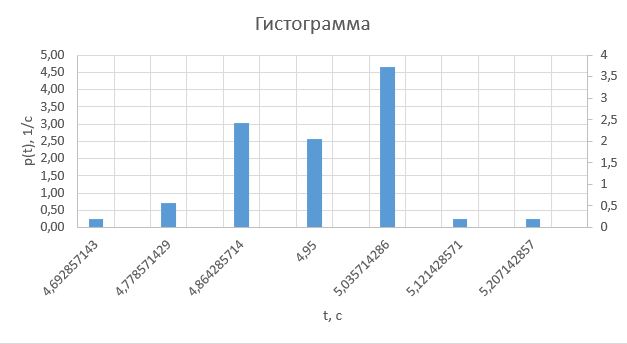
\includegraphics[width=10cm]{gysto.png}
\end{center}
\subsection{График плотности распределения}
\begin{center}
    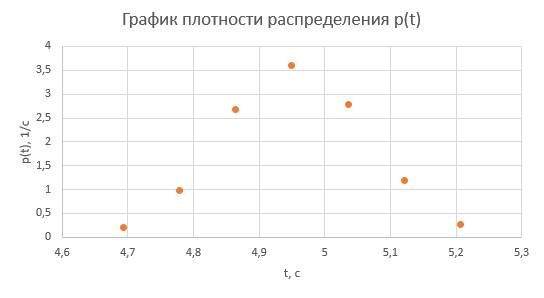
\includegraphics[width=10cm]{graph.png}
\end{center}
\section{Окончательные результаты}
Выполняя работу мы провели серию из 50 измерений по 5 секунд с использованием механического и электронного секундомера. Наглядно увидеть полученную статистику можно на графике плотности распределения и гистограмме
\end{document}
